\documentclass{standalone}
\usepackage{tikz,color}
\begin{document}

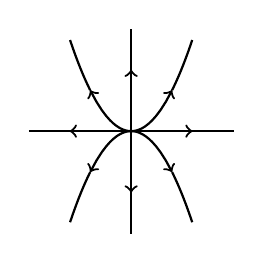
\begin{tikzpicture}[scale=1.3]
\draw [->,thick] (0,0) to (-0.6,0);
\draw [->,thick] (0,0)  to (0.6,0);
\draw [-,thick ] (-1,0) to (1,0);
\draw [->,thick] (0,0) to (0,0.6);
\draw [->,thick] (0,0)  to (0,-0.6);
\draw [-,thick ] (0,-1) to (0,1);
\draw [->,thick, domain=-4:0, samples=25] plot({0.4*exp(\x)},{0.4*exp(2*\x)});
\draw [-,thick, domain=  0:0.4, samples=25] plot({0.4*exp(\x)},{0.4*exp(2*\x)});
\draw [->,thick, domain=-4:0, samples=25] plot({-0.4*exp(\x)},{0.4*exp(2*\x)});
\draw [-,thick, domain=  0:0.4, samples=25] plot({-0.4*exp(\x)},{0.4*exp(2*\x)});
\draw [->,thick, domain=-4:0, samples=25] plot({0.4*exp(\x)},{-0.4*exp(2*\x)});
\draw [-,thick, domain=  0:0.4, samples=25] plot({0.4*exp(\x)},{-0.4*exp(2*\x)});
\draw [->,thick, domain=-4:0, samples=25] plot({-0.4*exp(\x)},{-0.4*exp(2*\x)});
\draw [-,thick, domain=  0:0.4, samples=25] plot({-0.4*exp(\x)},{-0.4*exp(2*\x)});

\end{tikzpicture}
\end{document}
